\afuncT{spline}{Interpolation using cubic splines.}{interpolation}
\\\cvsiplh
\afh
\\\hspace*{.04\textwidth} {
\ttfamily
\begin{tabular}[H]{|l|}
\multicolumn{1}{c}{
\Ts\rmfamily \bfseries Create Spline Object\vspace{.1cm}}\Bs\\ \hline
vsip\_spline\_d* vsip\_spline\_create\_d(vsip\_length);\Bs\\
vsip\_spline\_f* vsip\_spline\_create\_f(vsip\_length);\Bs\\
\hline\multicolumn{1}{c}{\Ts\rmfamily \bfseries Destroy Spline Object\vspace{.1cm}}\Bs\\ \hline
void vsip\_spline\_destroy\_d(vsip\_spline\_d*);\Bs\\
void vsip\_spline\_destroy\_f(vsip\_spline\_f*);\Bs\\
\hline\multicolumn{1}{c}{\Ts \rmfamily \bfseries Vector Splines\vspace{.1cm}}\Bs\\ \hline
void vsip\_vinterp\_spline\_d(const vsip\_vview\_d*, const vsip\_vview\_d*,
\fbrk{}vsip\_spline\_d*, const vsip\_vview\_d*, const vsip\_vview\_d*);\Bs\\
void vsip\_vinterp\_spline\_f(const vsip\_vview\_f*, const vsip\_vview\_f*,
\fbrk{}vsip\_spline\_f*, const vsip\_vview\_f*, const vsip\_vview\_f* ) ;\Bs\\
\hline\multicolumn{1}{c}{\Ts \rmfamily \bfseries Matrix Splines by Row or by Column\vspace{.1cm}}\Bs\\ \hline
void vsip\_minterp\_spline\_d(\fbrk{}const vsip\_vview\_d*, const vsip\_mview\_d*,
vsip\_spline\_d*,\fbrk{}vsip\_major,const vsip\_vview\_d*, const vsip\_mview\_d*);\Bs\\
void vsip\_minterp\_spline\_f(\fbrk{}const vsip\_vview\_f*, const vsip\_mview\_f*,
vsip\_spline\_f*,\fbrk{}vsip\_major, const vsip\_vview\_f*, const vsip\_mview\_f*);\Bs\\\hline
\end{tabular}
}\vspace*{3mm}
\\\pyjvsiph
\viewmthd{No}{No}{NA}{NA}
\apyclass{Yes}
%Example
\inputminted[linenos=true,resetmargins=true,xleftmargin=.12\textwidth,fontfamily=tt,fontsize=\small]{python}{./pyJvsip_examples/eXspline.py}
\hspace*{.08\textwidth}{\rmfamily For result see figure \ref{fig:SplineExample}.}\\
\begin{minipage}[c]{\textwidth}\centering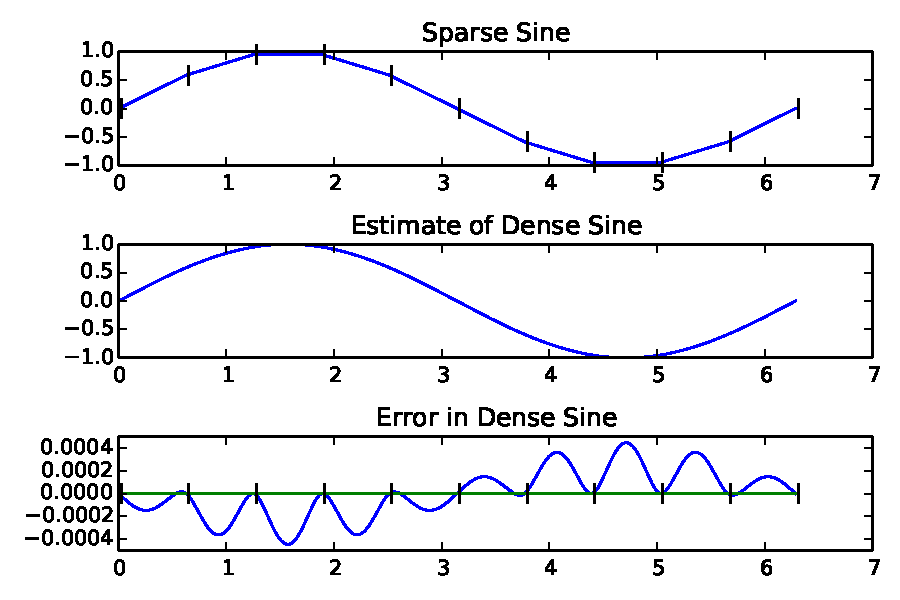
\includegraphics[width=0.8\textwidth]{./pyJvsip_examples/eXspline}\captionof{figure}{Spline Example}
\label{fig:SplineExample}\end{minipage}
%Instantiation
%Methods
\pyComment{\item{No comment}}